\section{Results}
\note{This section includes all results of running the simulation, with reports of expected time to detection being primary focus}


\note{from c\&B analysis of sequential decision making}
\note{Consider the following setting, where a single stationary tar-get is possibly located in a10×10 search region that is depicted in Fig. 5. The initial aggregate beliefB(0) is distributed among theC= 100 cells,  where  the  height  of  the  bars  in  each  cell represents the individual cell belief values, i.e., the probabilityp0cthat the target is present in a given cell, i.e.,c in {1,...,C} . SupposeB(0) = 0.75 ,  which  corresponds  to  an  initial  likeli-hood of 75\% that the target is truly present inA at the beginning of the search process. We examine the evolution of the search decision employing the different search strategies that are presented in the previous section. The search problem parameters that are used for the simulation studies, which are presented in this section, are tabu-lated in Table I. Simulations were allowed to run to completion (i.e., a decision was made), and statistics were calculated over N= 10 000 simulation replications. The values for the detec-tion errors, i.e.,alpha and beta , were chosen to reflect a representative sensor, such as a visual camera that provides aerial imagery in an outdoor and cluttered environment, which could be further calibrated empirically, e.g., by the sensor’s receiver operating characteristic (ROC) curve. Fig.  6  illustrates  the  evolution  of  the  belief  map  as  a search  agent  that  employs  the  myopic  search  strategy  thatmoves through the search region for the given search problem parameters. The searcher attempts to inspect or “clear” cells with the highest cell belief values, which, for the example bimodal belief distribution, requires visiting one peak followed by explo-ration of the other. Note that false-positive and false-negative detections  occur  throughout  the  search  process,  although  the searcher eventually arrives at the true location of the target and correctly terminates the search}


note{From C\&B Analysis of sequential decision-making using prob. search. Consider a bounded discretized search areaA , which is de-fined byC disjoint cells. This discrete representation can charac-terize numerous environment types of diverse spatial scale, such as open areas that are relevant to maritime search operations, cluttered regions, such as obstacle-filled arenas, or structured environments, such as rooms and hallways in a building. Other factors, which include the geometry and extent of the searcher’s sensor footprint, and the size of the sought object, or other op-erational considerations (e.g., existing coordinates or reference systems) can also govern the specific cellular decomposition of the search area}

\note{More general sensor models that account for additional spatial and/or temporal dependences be-cause  of  clutter  (indoor)  or  terrain  and  atmosphere  (outdoor) can  be  constructed  (e.g.,$\alpha$ s(k),kand $\beta$ s(k),k )  but  is  deferred for future study}


\note{In other words, the greater hindrance to deciding that a target is present in the search cell is the false-positive detection probabil-ity, since false alarms tend to prevent the searcher from “trust-ing” its positive observation. In contrast, if the missed detection probability is high, then the searcher cannot declare the search cell empty of the target with high confidence without expending multiple observations in the c}


The results presented in this section are generated by running monte carlo simulations, since finding a close-form solution to the expected time to decision (ETTD) is not readily available in the general case \cite{Chung2012AnalysisStrategies}. Following the approach outlined in \cite{Chung2007ASearch}, for each set of parameters in tables \ref{table:VaryingPriorDistribution}, \ref{table:VaryingInitialBelief}, \ref{table:MiscalibratedSensor}, \ref{table:MultipleTargetEGSweep}, \ref{table:MultipleTargetSaccadicRandom} and \ref{table:VaryingNumberOfAgents} we ran 5000 simulations. The parameters that we vary in the simulations are: 
\begin{enumerate}
    \item The prior belief distribution of each agent.
    \item The initial cumulative belief that the target is present in the region.
    \item The sensor model false positive rate and false negative rate.
    \item The number of targets present in the region.
    \item The number of agents participating in the search.
\end{enumerate}
The results of the simulation show the results of varying these parameters and suggest how to set them to achieve a desired result. We focus on the mostly commonly reported metrics in the literature, which are  related to the distribution of time to decision \cite{Chung2012AnalysisStrategies}, \cite{Waharte2010ProbabilisticRAVs}, \cite{Waharte2010SupportingRAVs}, \cite{Lau2007OptimalEnvironments}. We also report on the rate at which incorrect target locations are returned and the rate at which the agents incorrectly conclude that the target is not present. 

\par For each of the simulations, we arbitrarily chose to use the SPRT cutoff criteria with the upper Type \Romannum{1} error probability set to 0.1 and the upper Type \Romannum{2} error probability set to 0.15. In practice this meant the agent would terminate the search if its cumulative belief that the target was present exceeded $\approx$ 0.895 or subceeded $\approx$ 0.143. We generated simulated sensor readings using arbitrarily chosen values of the false positive rate = 0.2 and a false negative rate = 0.15. For each simulation run, we generated random starting locations for the agents and targets in a uniformly spaced 10 $\times$ 10 grid. Unless specified otherwise, we use the following default parameters: sensor model false negative rate = 0.15, sensor model false positive rate = 0.2, initial belief distribution = uniform, initial cumulative belief target is present = 0.5, number of targets present = 1, number of active agents = 1, the $\epsilon$-greedy search has $\epsilon$=0.2 and a neighborhood radius of 4. 

\subsection{Simulation Results Using a Single Agent}\label{subsec:SingleAgentSingleSourceResults}
\subsubsection{Varying the initial distribution of the agent belief}\label{subsubsec:VaryingPrior}

%\begin{landscape}
%\centering
%\vspace*{\fill}
\begin{table}[h!]
    \centering
    \begin{tabular}{| >{\centering} m{18mm} | >{\centering}m{22mm} | >{\centering}m{22mm} | >{\centering}m{22mm} | >{\centering}m{20mm} | m{20mm} <{\centering}|}
    \hline
       Strategy & Initial Belief Distribution & Mean TTD & Sample SD[TTD] & False Negative Rate & Proportion Incorrectly Localised \\
        \hline
        $\epsilon$-Greedy & Uniform & 112.93 & 62.38 & 0.152 & 0.040 \\
        $\epsilon$-Greedy & Gaussian & 21.68 & 20.44 & 0.0296 & 0.0118 \\
        \hline
        Sweep & Uniform & 601.57 & 183.45& 0.1254 & 0.0454 \\
        Sweep & Gaussian & 464.48 & 185.54 & 0.0832 & 0.0294 \\
        \hline
        Saccadic & Uniform & 98.83 & 56.13 & 0.1588 & 0.037 \\
        Saccadic & Gaussian & 14.558 & 18.75 & 0.0338 & 0.0114 \\
        \hline
        Random & Uniform & 629.55 & 282.95 & 0.1368 & 0.0336 \\
        Random & Gaussian & 501.83 & 268.45 & 0.0792 & 0.0308 \\
        \hline
    \end{tabular}
    \caption{Results of running the target localisation simulation with a Uniform initial belief distribution and Gaussian initial belief distribution for each implemented search strategy.}
    \label{table:VaryingPriorDistribution}
\end{table}
    
Table \ref{table:VaryingPriorDistribution} displays the results of running a simulation with a single agent and a single target while varying the initial belief distribution that the target is present in the search region. 
%The following parameters are fixed: Simulated Sensor False Negative Rate = 0.15, Simulated Sensor False Positive Rate = 0.2, Sensor model False Negative Rate = 0.15, Sensor Model False Positive Rate = 0.2, Initial belief that target is present in region = 0.5, SPRT Type \Romannum{1} error rate = 0.1, SPRT Type \Romannum{2} error rate = 0.15.
%\begin{itemize}
%    \item Simulated Sensor False Negative Rate = 0.15
%    \item Simulated Sensor False Positive Rate = 0.2
%    \item Sensor model False Negative Rate = 0.15
%    \item Sensor Model False Positive Rate = 0.2
%    \item Initial belief that target is present in region = 0.5
%    \item SPRT T\Romannum{1} error rate = 0.1, SPRT T\Romannum{2} error rate = 0.15.
%\end{itemize}
\begin{figure}
\centering
    \subfloat[Uniform initial belief distribution]{{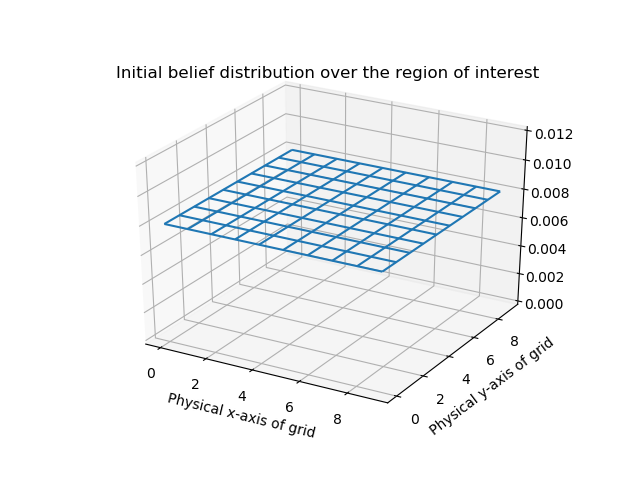
\includegraphics[width=6cm]{Chapters/MultiAgentTargetDetection/Figs/Results/Prior/Uniform/UniformInitialDistribution.png} }}%
    \qquad
    \subfloat[Gaussian initial belief distribution]{{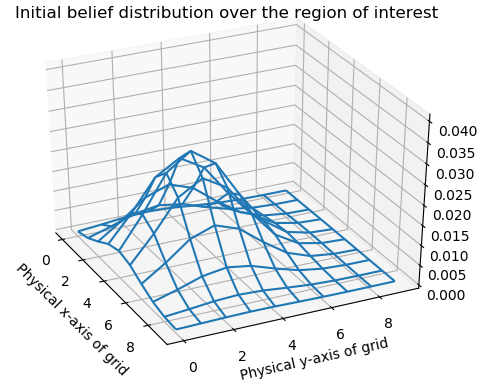
\includegraphics[width=6cm]{Chapters/MultiAgentTargetDetection/Figs/Results/Prior/Gaussian/GaussianInitialDistribution.png} }}%
    \caption{Initial belief distributions}%
    \label{fig:initialBeliefDistribution}%
\end{figure}
For each search strategy, we ran the simulation with both a Uniform and Gaussian initial belief distribution. The Gaussian mean coincided with the target location and the covariance matrix was $\begin{pmatrix} 3 & 0\\ 0 & 3\end{pmatrix}$, which is visualised in Figure \ref{fig:initialBeliefDistribution}. This represents a correct suspicion about the location of the target, which is the case in many scenarios where some prior information may suggest clues to the target location. As expected, for all of the search strategies the expected time until a decision reduces dramatically when using the Gaussian prior relative to the Uniform prior. 
%In the case of the two non-adaptive search methods (random and sweep), the effect is lessened as the search process is not influenced by new observations. 
Since the shape of the Gaussian distribution is aligned more closely to the true distribution that the Uniform distribution, it takes fewer samples to reach a sufficiently peaked distribution to reach the acceptance region for the SPRT. 
%This is visible by examining the evolution of the cumulative agent belief that the target is present in the region, shown in figures x and y.

\par It can also be seen that the false negative rate (the rate at which the agent incorrectly concludes that the target is not present in the region) drops in the case of the Gaussian prior relative to the uniform prior. This is also a result of using a prior distribution that matches the shape of the true distribution, since it requires a significant number of false positive/negative samples to modify the distribution enough to reach a negative conclusion.

%This is due to the unbiased sampling method of the non-adaptive strategies, which 

%but is higher for the non-adaptive search strategies since they are unbiased while sampling grid locations.
   

%    \hline
%    \multicolumn{2}{c}{Initial Discretised Gaussian Distribution of Belief Over Grid Cells (random mean, covariance matrix = [[], []]}\\
%    \hline

%\textbf{Gaussian Initial Belief Distribution (Mean coinciding with true target location)}
%\begin{table}[h!]
%    \centering
%    \begin{tabular}{| >{\centering} m{18mm} | >{\centering}m{20mm} | >{\centering}m{18mm} | >{\centering}m{20mm} | >{\centering}m{20mm} | m{20mm} <{\centering}|}
%    \hline
%       Strategy & Initial Belief Distribution & E[Time To Decision] & SD[Time To Decision] & False Negative Rate & Proportion Incorrect Localised \\
%        \hline
%        $\epsilon$ -Greedy & Gaussian & 21.68 & 20.44 & 0.0296 & 0.0118 \\
%        Sweep & Gaussian & 464.48 & 185.54 & 0.0832 & 0.0294 \\
%        Saccadic & Gaussian & 14.558 & 18.75 & 0.0338 & 0.0114 \\
%        Random & Gaussian & 501.83 & 268.45 & 0.0792 & 0.0308 \\
%    \hline
%    \end{tabular}

%  \caption{Results of running the target localisation simulation with a  uniform initial belief distribution and Gaussian initial belief distribution. p(T \Romannum{1}) = The probability of making a type \Romannum{1} error using the SPRT, p(T \Romannum{2}) = The probability of making a type \Romannum{1} error using the SPRT, Sim. FPR = The simulated false positive rate of the sensor, Sim. FNR = The simulated false negative rate of the sensor, E[TTD] = The expected amount of timesteps until a decision is made, Prec. = precision, Rec. = Recall. }\label{table:PriorGaussian}
%\end{table}





%\begin{landscape}

%\end{landscape}



































\break

\subsubsection{Varying the cumulative initial belief that the target is present in the search region}\label{subsubsec:VaryingPrior}
This experiment explored the consequences of varying the initial cumulative probability that the source is present. The cumulative probability of target presence reflects knowledge of likely the target presence is, prior to any evidence being gathered. We chose the parameters to reflect the cases where the search team do not believe it is unlikely that the target is present (0.25), it is equally likely that it is present as not present (0.5) and that it is likely that the target is present (0.75).

\begin{table}[H]
    \centering
    \begin{tabular}{| >{\centering} m{18mm} | >{\centering}m{24mm} | >{\centering}m{18mm} | >{\centering}m{20mm} | >{\centering}m{20mm} | m{20mm} <{\centering}|}
    \hline
       Strategy & Initial Belief Target Present & Mean TTD & Sample SD[TTD] & False Negative Rate & Proportion Incorrectly Localised \\
        \hline
        $\epsilon$-Greedy & 0.25 & 87.6214 & 30.9801 & 0.487 & 0.009 \\
        $\epsilon$-Greedy & 0.5 & 112.93 & 62.38 & 0.152 & 0.040 \\
        $\epsilon$-Greedy & 0.75  & 114.9276 & 81.9386 & 0.0396 & 0.1346 \\
         \hline
        Sweep & 0.25 & 520.4050 & 212.5122 & 0.4292 & 0.0118 \\
        Sweep & 0.5 & 601.57 & 183.45& 0.1254 & 0.0454 \\
        Sweep & 0.75 & 485.3650 & 242.1377 & 0.0326 & 0.1586 \\
        \hline
        Saccadic & 0.25 & 75.8320 & 29.8345 & 0.5054 & 0.0064 \\
        Saccadic & 0.5 & 98.83 & 56.13 & 0.1588 & 0.037 \\
        Saccadic & 0.75 & 100.1332 & 74.3883 & 0.0392 & 0.1418 \\
        \hline
        Random & 0.25 & 539.3802 & 267.6280 & 0.4284 & 0.0074 \\
        Random & 0.5 & 629.55 & 282.95 & 0.137 & 0.0336 \\
        Random & 0.75 & 538.0904 & 325.6283 & 0.035 & 0.1538 \\

    \hline
    \end{tabular}

  \caption{Results of running the target localisation simulation with a varying cumulative initial belief that the target is present in the search region.}\label{table:VaryingInitialBelief}
\end{table}

\begin{figure}[H]
\centering
    \subfloat[Belief for sweep search prematurely drops below the lower SPRT threshold with initial cumulative belief 0.25.]{{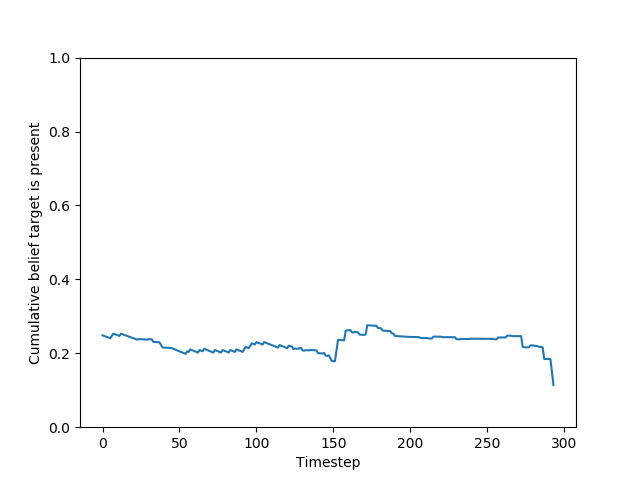
\includegraphics[width=7.4cm]{Chapters/MultiAgentTargetDetection/Figs/Results/BeliefEvolution/Sweep25InitialBelief/BeliefEvolution1.png} }}%
    \subfloat[Belief for sweep search does not prematurely drop below the lower SPRT threshold with initial cumulative belief 0.75.]{{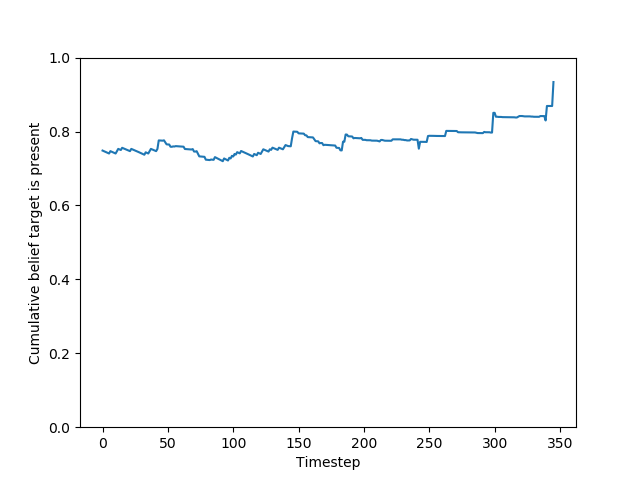
\includegraphics[width=7.4cm]{Chapters/MultiAgentTargetDetection/Figs/Results/BeliefEvolution/Sweep25InitialBelief/BeliefEvolution4.png} }}%
    \caption{Sample runs showing the effect of varying the agent's initial cumulative belief that the target is present}%
    \label{fig:initialCumulativeBelief}%
\end{figure}

Table \ref{table:VaryingInitialBelief} displays the results of running a simulation with a single agent and a single target while varying the agent's cumulative initial belief that the target is present in the search region. We discuss the results in relation to the adaptive and non-adaptive search methods:
\begin{enumerate}
    \item The results show that for the non-adaptive Sweep and Random search strategies, the mean TTD decreases when the initial belief that the target is present is set to both 0.25 and 0.75. In the case of the initial 0.25 belief value, the lower bound on the number of necessary observations before a conclusion can be drawn is found to be 62 consecutive negative observations at distinct locations. This would cause the SPRT to determine the target is not present. It is not likely for this to happen for the given parameters, since the sensor will generate false positive at a rate of 0.2, but there are much more likely scenarios that occur which cause the search to terminate early, for example observing 88 negative observations and 16 positive observations.
    %or 1 positive observation and 71 negative observations at distinct locations to pass the threshold(in the absence of any positive observations). Since there are 100 possible starting locations for the source, this is a likely scenario and
    \par The search terminates prematurely in a high proportion of cases, before a significant number of positive observations are observed to move the cumulative belief that the target is present away from the lower decision boundary. This can be observed in Figure \ref{fig:initialCumulativeBelief}, where on the left hand side there are not a sufficient number of positive observations to stop the search from terminating early. In the case of the 0.75 initial belief value, fewer positive observations are required to reach the upper termination criteria set by the SPRT compared to starting with an initial belief of 0.5, with the same phenomenon occurring for the belief starting at 0.25. In the best case, a starting belief of 0.25 would need 6 consecutive positive observations at the same location to cross the upper termination threshold, whereas a starting belief of 0.5 would  require 5 and a starting belief of 0.75 would only require 4. This comes at the price of making it easier to incorrectly identify the target location, increasing the proportion of runs where the target is incorrectly localised. 
    
    \item Relative to the cumulative belief starting at 0.5, the mean TTD only decreases for the adaptive $\epsilon$-greedy and Saccadic search methods in the case that the initial belief is 0.25 and slightly goes up for both in the case where it is 0.75. We had expected the mean time to decision to decrease in the case of the initial belief starting at 0.75 and increase in the case of the initial belief starting at 0.25, since they are respectively closer and further away from the upper SPRT decision boundary.
    %, due to the fact that it should require more samples to reach a positive conclusion. 
    The reason for the reduced mean TTD with an initial belief of 0.25 for the adaptive search methods is the same as that for the non-adaptive search methods, where the relatively large number of negative samples drove the cumulative belief below the lower SPRT threshold prematurely. The answer to the question of why the mean time to decision is less than that for the non-adaptive search methods lies with the biased sampling nature of the adaptive methods. If one of the adaptive methods comes across a spurious positive, the next choice of sample location will be the same (or probably be the same in the $\epsilon$-greedy case).
    \par For the parameters in this run of the simulation, after one positive spurious observation and one subsequent negative observation in the same location, the agent's belief that the target is present would be 0.2496. For the same scenario in the non-adaptive case, the agent would not re-sample the location with the spurious positive observation, but would continue on to sample the next location, which is likely to be a negative observation. In this case, the agent's belief that the target is present would be 0.2545, which is significantly higher than the adaptive case of 0.2496. Since the adaptive agent will re-sample spurious positives, it is able to then rule them out more quickly as potential target locations and as a result the expected time to decision is much lower than that for the non-adaptive methods. The slight increase in the TTD in the case where the initial belief is set to 0.75 is due to the large number of samples needed to break the lower threshold for the SPRT. For the cases where the initial belief set to 0.5 and 0.75, five and four consecutive positive observations at the same location are needed to cross the upper threshold respectively. 139 consecutive negative observations (100 at distinct locations, 39 at previously observed locations) would be needed to cross the lower threshold in the case of starting with an initial cumulative belief of 0.5 whereas 200 consecutive negative observations (100 distinct locations with 2 observations each) would be needed to cross the lower threshold in the case of starting with an initial cumulative belief of 0.75. The mean time to reach a negative decision was 309.1111 and 293.7143 for the $\epsilon$-greedy and saccadic cases with initial belief 0.75, compared to 196.6622 and 177.3552 with initial belief 0.5. The mean time to reach a positive decision was 106.9209 and 92.2352 for the $\epsilon$-greedy and saccadic cases with initial belief 0.75, compared to 97.9630 and 84.0031 with initial belief 0.5. 
    %The significantly longer time needed to reach a negative conclusion accounts for the slightly longer time to reach a decision when the initial belief is set to 0.5.
\end{enumerate}


%Really what want to say is that it takes 4 positive obs in same location to reach a decision and mean ttd for e greedy, saccadic are 97.96298915605847/196.6622691292876 and 84.00309082263433/177.3551637279597 with init 0.5 compared to 106.92086630570596/309.1111111111111 and 92.23522064945878/293.7142857142857










\break


\subsubsection{Varying the sensor model parameters}\label{subsubsec:MicalibratedSensor}

\begin{table}[h!]
    \centering
    \begin{tabular}{| >{\centering} m{18mm} | >{\centering}m{15mm} | >{\centering}m{15mm} | >{\centering}m{18mm} | >{\centering}m{18mm} | >{\centering}m{18mm} | m{19mm} <{\centering}|}
    \hline
       Strategy & Sensor Model FPR & Sensor Model FNR & Mean TTD & Sample SD[TTD] & False Negative Rate & Proportion Incorrectly Localised \\
        \hline
        $\epsilon$-Greedy & 0.05 & 0.02 & 67.2488 & 43.2448 & 0.1368 & 0.4270 \\
        $\epsilon$-Greedy & 0.2 & 0.15 & 112.9258 & 62.3798 & 0.1516 & 0.0398 \\
        $\epsilon$-Greedy & 0.4 & 0.4 & 197.5886 & 113.1707 & 0.0008 & 0.0000 \\
        \hline

        Saccadic & 0.05 & 0.02 & 59.9230 & 38.6500 & 0.1440 & 0.4298 \\
        Saccadic & 0.2 & 0.15 & 98.8274 & 56.1298 & 0.1588 & 0.0370 \\
        Saccadic & 0.4 & 0.4 & 142.2648 & 96.2213 & 0.0006 & 0.0 \\
        \hline
        
        Random & 0.05 & 0.02 & 167.2306 & 134.0652 & 0.015 & 0.7044 \\
        Random & 0.2 & 0.15 & 629.5462 & 282.9514 & 0.1368 & 0.0366 \\
        Random & 0.4 & 0.4 & 2100.5140 & 659.7263 & 0.1682 & 0.0 \\
        \hline
        
        Sweep & 0.05 & 0.02 & 132.1120 & 74.3178 & 0.0162 & 0.7932 \\
        Sweep & 0.2 & 0.15 & 601.5697 & 183.4529 & 0.1254 & 0.0454 \\
        Sweep & 0.4 & 0.4 & 2138.6002 & 554.5915 & 0.1344 & 0.0 \\
        \hline
        
    \end{tabular}

  \caption{Results of running the target localisation simulation with varying sensor model parameters for each implemented search strategy.}
  \label{table:MiscalibratedSensor}
\end{table}
\begin{figure}
\centering
    \subfloat[Sample run using Sweep search strategy]{{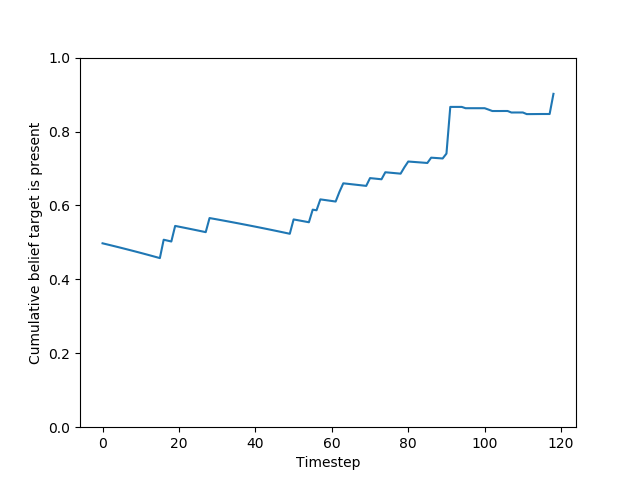
\includegraphics[width=6cm]{Chapters/MultiAgentTargetDetection/Figs/Results/BeliefEvolution/MiscalibratedSensor/05-02/SweepBeliefEvolution4.png}}}%
    \qquad
    \subfloat[Sample run using Saccadic search strategy]{{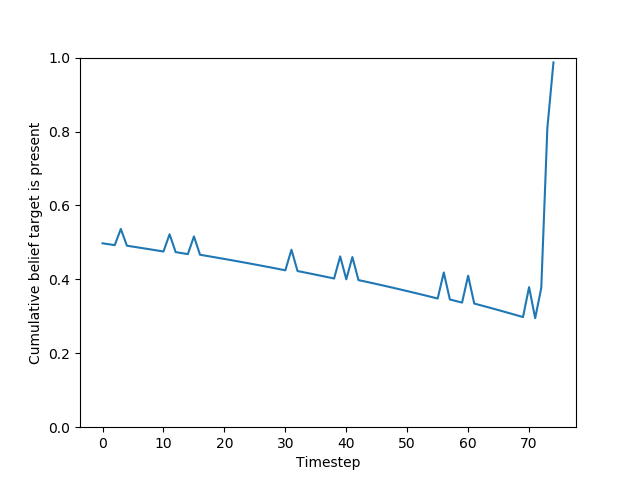
\includegraphics[width=6cm]{Chapters/MultiAgentTargetDetection/Figs/Results/BeliefEvolution/MiscalibratedSensor/05-02/SaccadicBeliefEvolution4.png} }}%
    \caption{Sample runs with miscalibrated sensor model parameters fpr=0.05, fnr=0.02}%
    \label{fig:MiscalibratedSensorFPR005}%
\end{figure}

\begin{figure}
\centering
    \subfloat[Sample run using Random search strategy]{{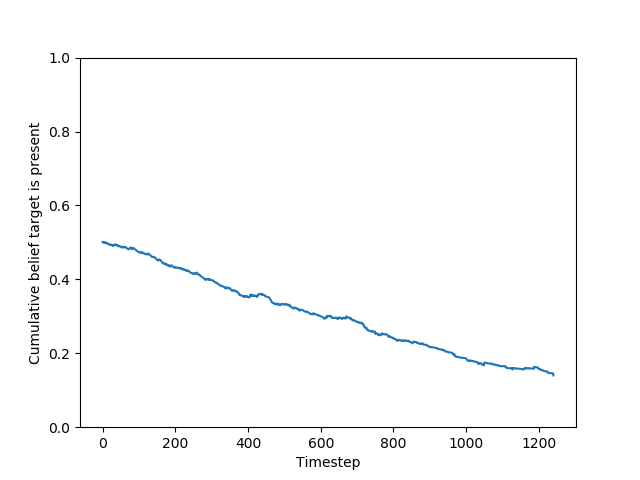
\includegraphics[width=6cm]{Chapters/MultiAgentTargetDetection/Figs/Results/BeliefEvolution/MiscalibratedSensor/4-4/RandomBeliefEvolution2.png}}}%
    \qquad
    \subfloat[Sample run using Saccadic search strategy]{{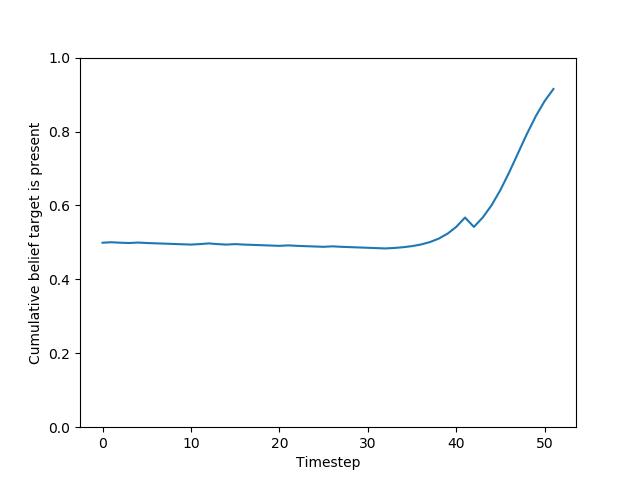
\includegraphics[width=6cm]{Chapters/MultiAgentTargetDetection/Figs/Results/BeliefEvolution/MiscalibratedSensor/4-4/SaccadicBeliefEvolution0.png} }}%
    \caption{Sample runs with miscalibrated sensor model parameters fpr=0.4, fnr=0.4}%
    \label{fig:MiscalibratedSensorFPR04}%
\end{figure}

Table \ref{table:MiscalibratedSensor} displays the results of running a simulation with a single agent and a single target while varying the parameters of the sensor model. The sensor model is parameterised using a false positive rate and false negative rate, detailed in equation \ref{eqn:EvidenceVarsProbs}. We deliberately chose extreme values for these parameters to show the effects of an extreme miscalibration, which can be thought of as a worst case scenario. We discuss the results in terms of underestimating and overestimating the true sensor parameters:
\begin{enumerate}
    \item When the model is calibrated to underestimate the rate at which the sensor will detect false negatives and false positives (the rows which have a sensor model fpr = 0.05, sensor model fnr = 0.02 in Table \ref{table:MiscalibratedSensor}), relative to the correctly calibrated sensor model (the rows which have a sensor model fpr = 0.2, sensor model fnr = 0.15 in Table \ref{table:MiscalibratedSensor}), both positive and negative observations will have a greater effect on the change in the shape of the distribution of the agent's belief, since the sensor model is more confident that the readings are correct. This means that is easier to cross the decision threshold of the SPRT due to spurious observations. For example, it would require 3, 5 and 17 positive consecutive observations at the same location to cross the upper SPRT threshold in the cases that the sensor model is calibrated with fpr=0.05/fnr=0.02, fpr=0.2/fnr=0.15, fpr=0.4/fnr=0.4 respectively.
    Underestimating the true sensor parameters leads to a much higher incorrect localisation rate in the adaptive search strategies in relation to the non-adaptive search strategies, which is evident in the Proportion Incorrectly Localised column of Table \ref{table:MiscalibratedSensor}. The reason for this is that the non-adaptive search strategies do not follow up on positive observations. The agent belief increases a relatively large amount with every positive observation, which actually arrive at a much higher rate (0.2066) than the sensor is calibrated for (0.0593). For example, if the agent immediately makes a positive observation, its belief will jump from 0.5 to 0.5425. Figure \ref{fig:MiscalibratedSensorFPR005} (a) shows the evolution of the agent's cumulative belief that the target is present in the search region. Relatively large jumps in cumulative belief due to the miscalibrated sensor model are clearly visible. This is in contrast with the adaptive strategies, where the agent re-samples positive observations, which drives the agent's belief back down in the case of spurious positives, which is visible in Figure \ref{fig:MiscalibratedSensorFPR005} (b).
    
    %\textit{Proportion Incorrectly Localised} column of table \ref{table:MiscalibratedSensor}. Similarly, we see that the false negative rate increases, as the miscalibrated model causes the belief in the target being absent for the region to increase more sharply with negative observations than the correctly calibrated sensor model. The mean time to decision (TTD) increases in this case because the belief in the target presence jumps disproportionately when a positive observation is made relative to a negative observation. The ratio of the sensor model FPR to FNR is approximately half the true ratio, which means the effect of positive observations is underestimated, causing the agent to delay the conclusion in a positive target localisation.
    \item Conversely, when the model is calibrated to overestimate the rate at which the sensor will record false positives and false negatives (the rows which have a sensor model fpr = 0.4, sensor model fnr = 0.4 in Table \ref{table:MiscalibratedSensor}), the belief distribution changes much more gradually given positive or negative observations. This means that crossing the decision thresholds given by the SPRT will require many more positive or negative readings, which leads to much higher mean times to decision (TTD) for all search strategies. As a lower bound, the SPRT would require 447 consecutive negative observations when running the sweep search in order to conclude that the target is not present. In the adaptive cases, once a positive observation is made at a given location, the agent's belief usually becomes highest at that location, which causes the agent to sample there again. Once it visits the true target location, usually it will receive a sufficient number of positive observations to keep sampling it, which causes its cumulative belief to steadily increase, as shown in Figure \ref{fig:MiscalibratedSensorFPR04} (a). The non-adaptive methods do not exhibit this behaviour since they are unbiased sampling methods. They do not re-sample when they come across a positive observation, which causes their cumulative belief in the target presence to gradually drop. If they do not experience consecutive positive observations when they visit the true target location, usually their belief will drop below the SPRT threshold, as can be seen in Figure \ref{fig:MiscalibratedSensorFPR04} (b).
\end{enumerate}
\break

\subsubsection{Varying the number of targets present in the region}\label{subsubsec:VaryingNoTargets}
\begin{landscape}
\centering
\vspace*{\fill}
\begin{table}[h!]
    \centering
    \begin{tabular}{| >{\centering} m{18mm} | >{\centering}m{20mm} | >{\centering}m{18mm} | >{\centering}m{20mm} | >{\centering}m{20mm} | >{\centering}m{20mm} | m{60mm} <{\centering}|}
    \hline
       Strategy & Number of Targets Present & E[Time To Decision] & SD[Time To Decision] & False Negative Rate & Proportion Incorrect Localised & Decision Matrix\\
        \hline
        $\epsilon$ -Greedy & 1 & 112.93 & 62.38 & 0.152 & 0.040 & ToDo\\
        $\epsilon$ -Greedy & 2 & 155.77 & 50.93 & ToDo & ToDo & \begin{tabular}{l|l|c|c|c}
\multicolumn{2}{c}{}&\multicolumn{2}{c}{diagnosis}&\\
\cline{3-4}
\multicolumn{2}{c|}{}&0&1&\multicolumn{1}{c}{Total}\\
\cline{2-4}
\multirow{2}{*}{G}& 0 & $a$ & $b$ & $a+b$\\
\cline{2-4}
& 1 & $c$ & $d$ & $c+d$\\
\cline{2-4}
\multicolumn{1}{c}{} & \multicolumn{1}{c}{Total} & \multicolumn{1}{c}{$a+c$} & \multicolumn{    1}{c}{$b+d$} & \multicolumn{1}{c}{$N$}\\
\end{tabular} \\
        $\epsilon$ -Greedy & 3 & 175.84 & 42.78 & ToDo & ToDo & \begin{tabular}{l|l|c|c|c|}
\multicolumn{2}{c}{}&\multicolumn{2}{c}{\#Correct G}&\\
\cline{3-5}
\multicolumn{2}{c|}{}&0&1&2%\multicolumn{1}{c}{Total}
\\
\cline{2-5}
\multirow{2}{*}{\# G}& 0 & $a$ & $b$ & $c$\\
\cline{2-5}
& 1 & $e$ & $f$ & $g$\\
\cline{2-5}
& 2 & $h$ & $i$ & $j$\\
\cline{2-5}
\multicolumn{1}{c}{} & \multicolumn{1}{c}{Total} & \multicolumn{1}{c}{$x$} & \multicolumn{    1}{c}{$y$} & \multicolumn{1}{c}{$N$}\\
\end{tabular} \\
        \hline
        Sweep & 1 & 601.57 & 183.45 & 0.1254 & 0.0454  & ToDo\\
        Sweep & 2 & 708.02 & 206.57 & ToDo & ToDo  & ToDo\\
        Sweep & 3 & 770.00 & 223.96 & ToDo & ToDo & ToDo \\
        \hline
        Saccadic & 1 & 98.83 & 56.13 & 0.1588 & 0.037 & ToDo \\
        Saccadic & 2 & 135.64 & 45.43 & ToDo & ToDo & ToDo \\
        Saccadic & 3 & 154.59 & 36.62 & ToDo & ToDo & ToDo \\
        \hline
        Random & 1 & 629.55 & 282.95 & 0.1368 & 0.0336 & ToDo \\
        Random & 2 & 787.44 & 287.61 & ToDo & ToDo & ToDo \\
        Random & 3 & 882.74 & 295.05 & ToDo & ToDo & ToDo \\
        \hline
    \end{tabular}
    \caption{Results of running the target localisation simulation with a \textbf{varying number of targets}. Fixed P(T1) = 0.1, p(T2) = 0.15, Simulated Sensor FPR = 0.2, Simulated Sensor FNR = 0.15, Sensor Model FPR = 0.2, Sensor Model FNR = 0.15, }
    \label{table:PriorUniform}
\end{table}
\end{landscape}

\break

\begin{table}[h!]
    \centering
    \begin{tabular}{| >{\centering} m{17mm} | >{\centering}m{13mm} | >{\centering}m{14mm} | >{\centering}m{15mm} | m{72mm} <{\centering}|}
    \hline
       Strategy & \# Targets Present & E[TTD] & SD [TTD] & Decision Matrix Showing \# Returned Target Locations (Rows) vs. \# Targets Correctly Localised (Cols).\\
        \hline
        $\epsilon$ -Greedy & 1 & 112.93 & 62.38 & {
        \centering
        \begin{tabular}{c|c|c|}
           \multicolumn{1}{c}{} & \multicolumn{2}{c}{ } \\
           \multicolumn{1}{c}{} & \multicolumn{1}{c}{0}  & \multicolumn{1}{c}{1} \\
           \cline{2-3}
            0 & 0.152 & 0 \\ \cline{2-3}
            1 & 0.0400 & 0.8080 \\\cline{2-3}
            \multicolumn{3}{c}{}
        \end{tabular}
        }\\
        $\epsilon$ -Greedy & 2 & 155.77 & 50.93 & 
        {
        \centering
        \begin{tabular}{c|c|c|c|}
           \multicolumn{1}{c}{} & \multicolumn{3}{c}{ } \\
           \multicolumn{1}{c}{} & \multicolumn{1}{c}{0}  & \multicolumn{1}{c}{1}  & \multicolumn{1}{c}{2} \\
           \cline{2-4}
            0 & 0.0218 & 0 & 0 \\ \cline{2-4}
            1 & 0.0012 & 0.2644 & 0 \\\cline{2-4}
            2 & 0.0006 & 0.0474 & 0.6646 \\\cline{2-4}
        \end{tabular}
        }
        \\
        $\epsilon$ -Greedy & 3 & 175.84 & 42.78 &
        {
        \centering
        \begin{tabular}{c|c|c|c|c|}
           \multicolumn{1}{c}{} & \multicolumn{4}{c}{ } \\
           \multicolumn{1}{c}{} & \multicolumn{1}{c}{0}  & \multicolumn{1}{c}{1}  & \multicolumn{1}{c}{2}& \multicolumn{1}{c}{3} \\
           \cline{2-5}
            0 & 0.0038 & 0 & 0 & 0\\ \cline{2-5}
            1 & 0 & 0.0596 & 0 & 0 \\\cline{2-5}
            2 & 0 & 0.0064 & 0.3170 & 0\\\cline{2-5}
            3 & 0 & 0.0002 & 0.0510 & 0.5620\\\cline{2-5}
            \multicolumn{4}{c}{}\\
        \end{tabular}
        }
        \\
        \hline
        Sweep & 1 & 601.57 & 183.45 & {
        \centering
        \begin{tabular}{c|c|c|}
           \multicolumn{1}{c}{} & \multicolumn{2}{c}{ } \\
           \multicolumn{1}{c}{} & \multicolumn{1}{c}{0}  & \multicolumn{1}{c}{1} \\
           \cline{2-3}
            0 & 0.1254 & 0 \\ \cline{2-3}
            1 & 0.0454 & 0.8292 \\\cline{2-3}
            \multicolumn{3}{c}{}
        \end{tabular}
        }\\
        Sweep & 2 & 708.02 & 206.57 &
        {
        \centering
        \begin{tabular}{c|c|c|c|}
           \multicolumn{1}{c}{} & \multicolumn{3}{c}{ } \\
           \multicolumn{1}{c}{} & \multicolumn{1}{c}{0}  & \multicolumn{1}{c}{1}  & \multicolumn{1}{c}{2} \\
           \cline{2-4}
            0 & 0.0106 & 0 & 0 \\ \cline{2-4}
            1 & 0.0002 & 0.181 & 0 \\\cline{2-4}
            2 & 0.0018 & 0.0666 & 0.7398 \\\cline{2-4}
        \end{tabular}
        }
        \\
        Sweep & 3 & 770.00 & 223.96 & 
        {
        \centering
        \begin{tabular}{c|c|c|c|c|}
           \multicolumn{1}{c}{} & \multicolumn{4}{c}{ } \\
           \multicolumn{1}{c}{} & \multicolumn{1}{c}{0}  & \multicolumn{1}{c}{1}  & \multicolumn{1}{c}{2}& \multicolumn{1}{c}{3} \\
           \cline{2-5}
            0 & 0.002 & 0 & 0 & 0\\ \cline{2-5}
            1 & 0.0002 & 0.022 & 0 & 0 \\\cline{2-5}
            2 & 0 & 0.0014 & 0.2104 & 0\\\cline{2-5}
            3 & 0.0002 & 0.0034 & 0.082 & 0.6784\\\cline{2-5}
            \multicolumn{4}{c}{}
        \end{tabular}
        }
        \\
        \hline
        \end{tabular}
        \caption{Results of running the target localisation simulation with 1,2 and 3 targets for sweep search and $\epsilon$-greedy search.}
        \label{table:MultipleTargetEGSweep}
        \end{table}
        
        
        
        
        
        \begin{table}[h!]
        \begin{tabular}{| >{\centering} m{17mm} | >{\centering}m{13mm} | >{\centering}m{14mm} | >{\centering}m{15mm} | m{72mm} <{\centering}|}
        \hline
        Strategy & No. Targets Present & E[TTD] & SD [TTD] & Decision Matrix Showing \# Returned Target Locations (Rows) vs. \# Targets Correctly Localised (Cols).\\
        \hline
        Saccadic & 1 & 98.83 & 56.13 & {
        \centering
        \begin{tabular}{c|c|c|}
           \multicolumn{1}{c}{} & \multicolumn{2}{c}{ } \\
           \multicolumn{1}{c}{} & \multicolumn{1}{c}{0}  & \multicolumn{1}{c}{1} \\
           \cline{2-3}
            0 & 0.1588 & 0 \\ \cline{2-3}
            1 & 0.0370 & 0.8042 \\\cline{2-3}
            \multicolumn{3}{c}{}
        \end{tabular}
        } \\
        Saccadic & 2 & 135.64 & 45.43 & 
        {
        \centering
        \begin{tabular}{c|c|c|c|}
           \multicolumn{1}{c}{} & \multicolumn{3}{c}{ } \\
           \multicolumn{1}{c}{} & \multicolumn{1}{c}{0}  & \multicolumn{1}{c}{1}  & \multicolumn{1}{c}{2} \\
           \cline{2-4}
            0 & 0.0258 & 0 & 0 \\ \cline{2-4}
            1 & 0.0014 & 0.2664 & 0 \\\cline{2-4}
            2 & 0 & 0.0448 & 0.6616 \\\cline{2-4}
        \end{tabular}
        }
        \\
        Saccadic & 3 & 154.59 & 36.62 &
        {
        \centering
        \begin{tabular}{c|c|c|c|c|}
           \multicolumn{1}{c}{} & \multicolumn{4}{c}{ } \\
           \multicolumn{1}{c}{} & \multicolumn{1}{c}{0}  & \multicolumn{1}{c}{1}  & \multicolumn{1}{c}{2}& \multicolumn{1}{c}{3} \\
           \cline{2-5}
            0 & 0.0052 & 0 & 0 & 0\\ \cline{2-5}
            1 & 0.0002 & 0.07 & 0 & 0 \\\cline{2-5}
            2 & 0 & 0.0036 & 0.3246 & 0\\\cline{2-5}
            3 & 0 & 0.0006 & 0.0458 & 0.55\\\cline{2-5}
            \multicolumn{4}{c}{}
        \end{tabular}
        }
        \\
        \hline
        Random & 1 & 629.55 & 282.95 & {
        \centering
        \begin{tabular}{c|c|c|}
           \multicolumn{1}{c}{} & \multicolumn{2}{c}{ } \\
           \multicolumn{1}{c}{} & \multicolumn{1}{c}{0}  & \multicolumn{1}{c}{1} \\
           \cline{2-3}
            0 & 0.1368 & 0 \\ \cline{2-3}
            1 & 0.0336 & 0.8296 \\\cline{2-3}
            \multicolumn{3}{c}{}
        \end{tabular}
        } \\
        Random & 2 & 787.44 & 287.61 & 
        {
        \centering
        \begin{tabular}{c|c|c|c|}
           \multicolumn{1}{c}{} & \multicolumn{3}{c}{ } \\
           \multicolumn{1}{c}{} & \multicolumn{1}{c}{0}  & \multicolumn{1}{c}{1}  & \multicolumn{1}{c}{2} \\
           \cline{2-4}
            0 & 0.0166 & 0 & 0 \\ \cline{2-4}
            1 & 0.0012 & 0.1872 & 0 \\\cline{2-4}
            2 & 0.0004 & 0.053 & 0.7416 \\\cline{2-4}
        \end{tabular}
        }
        \\
        Random & 3 & 882.74 & 295.05 & 
        {
        \centering
        \begin{tabular}{c|c|c|c|c|}
           \multicolumn{1}{c}{} & \multicolumn{4}{c}{ } \\
           \multicolumn{1}{c}{} & \multicolumn{1}{c}{0}  & \multicolumn{1}{c}{1}  & \multicolumn{1}{c}{2}& \multicolumn{1}{c}{3} \\
           \cline{2-5}
            0 & 0.0014 & 0 & 0 & 0\\ \cline{2-5}
            1 & 0.0002 & 0.0248 & 0 & 0 \\\cline{2-5}
            2 & 0 & 0.0014 & 0.2138 & 0\\\cline{2-5}
            3 & 0 & 0.0022 & 0.0608 & 0.6954 \\\cline{2-5}
            \multicolumn{4}{c}{}
        \end{tabular}
        }
        \\
        \hline
    \end{tabular}
    \caption{Results of running the target localisation simulation with 1,2 and 3 targets for saccadic search and random search.}
    \label{table:MultipleTargetSaccadicRandom}
\end{table}

Tables \ref{table:MultipleTargetEGSweep} and \ref{table:MultipleTargetSaccadicRandom} display the results of running a simulation with a single agent with a varying number of targets in the search region. We ran algorithm \ref{alg:MultiTargetLocalisation} to carry out the localisation procedure. The results show that the mean time to decision increases sub-linearly with respect to the number of targets present. The rows of the decision matrix show the proportions of how many target locations are returned by the agent and the columns show how many targets are correctly localised. The results indicate that the more targets that are present, the less willing the agent is to conclude that the are no targets present, but that it is also less willing to conclude that the maximum number of targets are present. The reason why the agent consistently returns 0 target locations at a lower rate when there is more targets present can be explained by the miscalibrated sensor results; since there are more targets present, the number of observed true positives is greater than the calibrated values. This essentially means that the sensor model fnr is over-estimated, which leads to a much lower search false negative rate. This could be overcome by calibrating the sensor model with the fnr and fpr that would arise from the number of targets suspected to be present in the region, and re-calibrating it each time a target is localised by the agent.
\break


\subsection{Varying number of search agents}

This experiment explored how varying the number of agents involved in the search impacted on the effectiveness of the search. We assumed that agents communicated their most recent observation to all other agent at each time step, which the other agents used to update their local belief that the target it present in the region.


\begin{table}[H]
    \centering
    \begin{tabular}{| >{\centering} m{18mm} | >{\centering}m{20mm} | >{\centering}m{18mm} | >{\centering}m{20mm} | >{\centering}m{20mm} | m{20mm} <{\centering}|}
    \hline
       Strategy & \# Agents & Mean TTD & Sample SD[TTD] & False Negative Rate & Proportion Incorrectly Localised \\
        \hline
        $\epsilon$-Greedy & 1 & 112.9258 & 62.3798 & 0.1516 & 0.0398 \\
        $\epsilon$-Greedy & 2 & 65.5912 & 34.3248 & 0.1568 & 0.0314 \\
        $\epsilon$-Greedy & 3 & 47.5176 & 24.9861 & 0.1428 & 0.0262 \\
        \hline
        Sweep & 1 & 601.5697 & 183.4529 & 0.1254 & 0.0454 \\
        Sweep & 2  & 303.7328 & 94.2748 & 0.1232 & 0.0466 \\
        Sweep & 3 & 204.8172 & 65.1273 & 0.1252 & 0.0408 \\
        \hline
        Saccadic & 1 & 98.8274 & 56.1298 & 0.1588 & 0.0370 \\
        Saccadic & 2 & 75.3466 & 39.9718 & 0.1520 & 0.0132 \\
        Saccadic & 3 & 65.0774 & 33.9798 & 0.1598 & 0.0090 \\
        \hline
        Random & 1 & 629.5462 & 282.9514 & 0.1368 & 0.0366 \\
        Random & 2 & 315.0082 & 140.3954 & 0.1254 & 0.0366  \\
        Random & 3 & 211.4242 & 94.7801 & 0.1222 & 0.0448\\
        \hline
    \end{tabular}
   \caption{Results of running the target localisation simulation with a varying number of homogeneous agents for each implemented search strategy.}
    \label{table:VaryingNumberOfAgents}
\end{table}

Table \ref{table:VaryingNumberOfAgents} shows the results of running the search with 1, 2 and 3 homogeneous agents. Each agent is initialised with the same parameters, but start at independently chosen random locations. They receive new observations from other agents at each time-step and then record their own observation. We did not assume that there could be corrupted/interrupted transmissions, although this could be investigated in future work.
%The results agree closely with \cite{Chung2008Multi-agentFramework}. 
Figure 2 and Figure 3 of \cite{Chung2008Multi-agentFramework} show sample runs of adaptive and non-adaptive search strategies for the same simulation configuration. The observed results matched our expectations based on \cite{Chung2008Multi-agentFramework}, where the largest relative reduction in the mean TTD is found in the non-adaptive cases. This is because the non-adaptive cases use unbiased sampling methods. The sweep search method samples all grid cells an equal number of times, so running multiple agents is equivalent to running a single agent with the non-adaptive strategy that can sample multiple times on each time-step rather than just once. This implies the search time is inversely proportional to the number of agents used in the non-adaptive cases, supported by Table \ref{table:VaryingPriorDistribution}. Since the agents first record a sensor observation and update their belief before updating their belief based on other agent observations made at the current time-step, sometimes an agent will end its search before the other agents, which means that the effect of having multiple agents is lessened. This is more prevalent when using the adaptive strategies since when the agents locate the source correctly, there is a chance that one could receive a false negative, while the others terminate with true positive observations. This leads the last agent to make extra observations, inflating the mean TTD. The unbiased methods do not exhibit this behaviour as much and usually terminate when one agent at the target location makes a positive observation which is shared among other agents who are not at the target location and who then also subsequently terminate.


